\documentclass[a4paper,14pt]{extarticle}
%\documentclass[a4paper]{article}
\usepackage[T2A]{fontenc}
\usepackage[utf8]{inputenc}
\usepackage[english,russian]{babel}
\usepackage{indentfirst}
\usepackage{amssymb}
\usepackage{amsfonts}
\usepackage{amsmath}
\usepackage{mathtext}
\usepackage{cite}
\usepackage{enumerate}
\usepackage{float}
\usepackage[top=1.5cm,bottom=1.5cm,left=2.5cm,right=1.5cm]{geometry}
\usepackage[unicode]{hyperref}
\usepackage{graphicx}
\usepackage{color}
\usepackage[colorinlistoftodos]{todonotes}
\usepackage[format=hang, labelsep=period, margin=8pt, figurename=Рис.]{caption}
\usepackage{listings}
\usepackage{subcaption}
%\usepackage{showkeys}
\usepackage[onehalfspacing, nodisplayskipstretch]{setspace}

\definecolor{dkgreen}{rgb}{0,0.6,0}
\definecolor{gray}{rgb}{0.5,0.5,0.5}
\definecolor{mauve}{rgb}{0.58,0,0.82}

\numberwithin{equation}{section}
\setcounter{secnumdepth}{3} % глубина нумеруемых разделов
\setcounter{tocdepth}{3} % глубина оглавления

\begin{document}
%\listoftodos
%\clearpage
\newpage
\begin{titlepage}
\newpage

\begin{center}
	Министерство образования и науки Российской Федерации \\
	МОСКОВСКИЙ ФИЗИКО-ТЕХНИЧЕСКИЙ ИНСТИТУТ\\(государственный университет)\\[0.5cm]
	ФАКУЛЬТЕТ АЭРОФИЗИКИ И КОСМИЧЕСКИХ ИССЛЕДОВАНИЙ\\
	КАФЕДРА ВЫЧИСЛИТЕЛЬНОЙ МАТЕМАТИКИ\\
	(Специализация «Компьютерное моделирование\\
	в механике, биомеханике и физиологии»)\\[1cm]
\end{center}

\vspace{1em}

\begin{center}
	\textsc{\textbf{Численное моделирование\\
	 сеточно-характеристическим методом\\
	 волновых процессов при неразрушающем контроле\\
	 изделий из изотропных и анизотропных\\
	 композитных материалов}}\\[2cm]
	Магистерская диссертация\\[0.5cm]
	студента 031 группы\\
	Казакова Александра Олеговича\\
\end{center}

\vspace{1.5em}

\begin{center}
	Научный руководитель\\
	Васюков Алексей Викторович, к.ф.-м.н.
\end{center}

%\vspace{3.5em}
\vfill

\begin{center}
	г.Долгопрудный\\
	2016
\end{center}


\end{titlepage}

\setcounter{page}{2}
\tableofcontents
\clearpage
\newpage
\section*{Введение}
\addcontentsline{toc}{section}{Введение}
В данной работе рассматривается численное моделирование волновых деформационных процессов в твёрдых телах. Для описание физических процессов используются уравнения на скорости и напряжения в частицах материала из механики сплошной среды для деформируемого твёрдого тела. Рассчёт имеющейся системы уравнений проводится численно сеточно-характеристическим методом с расщеплением по трём пространственным направлениям. Он позволяет получать динамическую волновую картину.


\begin{itemize}
\item а
\item б
\item в
\item г
\end{itemize}

\clearpage
\newpage
\section*{Глава 1\\Основные уравнения механики деформируемого твёрдого тела}
\addcontentsline{toc}{section}{Глава 1. Основные уравнения механики деформируемого твёрдого тела}
\setcounter{section}{1}
\setcounter{subsection}{0}
\setcounter{equation}{0}

\subsection{Уравнения механики деформируемого твёрдого тела}
	
	Основные определяющие соотношения МДТТ включают в себя уравнения движения и реологические соотношения \cite{novatsky,sedov,rabotnov}.
	Посление определяют сопротивление материала по отношению к внешнему воздействию.
\begin{align}
	\label{initial_equations}
	\rho\dot{v}_i &= \nabla_j\sigma_{ij}+f_i & \textrm{(уравнения движения)}\nonumber\\
	\dot{\sigma}_{ij} &= q_{ijkl}\dot{\varepsilon}_{kl}+F_{ij} & \textrm{(реологические соотношения).}
\end{align}
	Здесь $\rho$ – плотность среды, $v_i$ – компоненты скорости смещения,
	$\sigma_{ij}$, $\varepsilon_{ij}$ -- компоненты тензоров напряжений и деформаций,
	$\nabla_j$ – ковариантная производная по $j$-й координате, $f_i$ – массовые
	силы, действующие на единицу объёма, $F_{ij}$ -- правая часть, используемая, например, для описания диссипации в моделях с учётом вязкости.

	В случае малых деформаций тензор скоростей деформаций $e_{ij}=\dot{\varepsilon}_{ij}$ 
	выражается через компоненты скорости смещения линейным образом \cite{landau_lifshits}:
	
\begin{equation}
	\label{small_deformation}
	e_{ij}=\frac{1}{2}(\nabla_j v_i+\nabla_i v_j).
\end{equation}

	Вид компонент тензора 4-го порядка $q_{ijkl}$ и правой части $F_{ij}$ определяется реологией среды.

	Для замыкания системы уравнений \eqref{initial_equations} её необходимо дополнить уравнением состояния, определяющим зависимость плотности от напряжений:

\begin{equation}
	\rho=\rho_0e^{\frac{p}{K}},
\end{equation}
	где $p=-\frac{1}{3}\sum\sigma_{kk}$ -- давление, $K=\lambda+\frac{2}{3}\mu$ -- коэффициент всестороннего сжатия, $\lambda$ и $\mu$ -- параметры Ламе.

	Параметры Ламе зависят от материала и связаны с модулем продольной упругости и коэффициентом Пуассона следующим образом:
\begin{align}
	\label{lame_parameters}
	\lambda &= \frac{E\nu}{(1+\nu)(1-2\nu)}
	\nonumber\\
	\mu &= G=\frac{E}{2(1+\nu)}.
\end{align}
	Здесь $E$ -- модуль продольной упругости, $\nu$ -- коэффициент Пуассона, $G$ -- модуль сдвига.
\clearpage
\newpage

\subsection{Приближение линейно упругого тела}
	
	В простейшем случае линейной упругости тензор $q_{ijkl}$ и правая часть $F_{ij}$ в \eqref{initial_equations} принимают следующий вид \cite{landau_lifshits}:
\begin{align}
	\label{tensor_qijkl_elastic}
	q_{ijkl}&=\lambda\delta_{ij}\delta_{kl}+\mu(\delta_{ik}\delta_{jl}+\delta_{il}
	\delta_{jk}),\nonumber\\
	F_{ij}&=0.
\end{align}
	В этом соотношении $\lambda$ и $\mu$ -- параметры Ламе, $\delta_{ij}$ -- символ Кронекера.
	
	Уравнения \eqref{initial_equations} в приближении \eqref{small_deformation} будут выглядеть следующим образом: 
\begin{align}
	\label{simple_equations}
	\frac{\partial{v_x}}{\partial{t}}&=\frac{1}{\rho}(\frac{\partial{\sigma_{xx}}}{\partial{x}}+\frac{\partial{\sigma_{xy}}}{\partial{y}}+\frac{\partial{\sigma_{xz}}}{\partial{z}})
	\nonumber\\
	\frac{\partial{v_y}}{\partial{t}}&=\frac{1}{\rho}(\frac{\partial{\sigma_{xy}}}{\partial{x}}+\frac{\partial{\sigma_{yy}}}{\partial{y}}+\frac{\partial{\sigma_{yz}}}{\partial{z}})
	\nonumber\\
	\frac{\partial{v_z}}{\partial{t}}&=\frac{1}{\rho}(\frac{\partial{\sigma_{xz}}}{\partial{x}}+\frac{\partial{\sigma_{yz}}}{\partial{y}}+\frac{\partial{\sigma_{zz}}}{\partial{z}})
	\nonumber\\
	\frac{\partial{\sigma_{xx}}}{\partial{t}}&=(\lambda+2\mu)\frac{\partial{v_x}}{\partial{x}}+\lambda\frac{\partial{v_y}}{\partial{y}}+\lambda\frac{\partial{v_z}}{\partial{z}}
	\nonumber\\
	\frac{\partial{\sigma_{xy}}}{\partial{t}}&=\mu(\frac{\partial{v_x}}{\partial{y}}+\frac{\partial{v_y}}{\partial{x}})
	\nonumber\\
	\frac{\partial{\sigma_{xz}}}{\partial{t}}&=\mu(\frac{\partial{v_x}}{\partial{z}}+\frac{\partial{v_z}}{\partial{x}})
	\nonumber\\
	\frac{\partial{\sigma_{yy}}}{\partial{t}}&=\lambda\frac{\partial{v_x}}{\partial{x}}+(\lambda+2\mu)\frac{\partial{v_y}}{\partial{y}}+\lambda\frac{\partial{v_z}}{\partial{z}}
	\nonumber\\
	\frac{\partial{\sigma_{yz}}}{\partial{t}}&=\mu(\frac{\partial{v_z}}{\partial{y}}+\frac{\partial{v_y}}{\partial{z}})
	\nonumber\\
	\frac{\partial{\sigma_{zz}}}{\partial{t}}&=\lambda\frac{\partial{v_x}}{\partial{x}}+\lambda\frac{\partial{v_y}}{\partial{y}}+(\lambda+2\mu)\frac{\partial{v_z}}{\partial{z}}
\end{align}

	Обозначив искомый вектор $\vec{u}=\{v_x,v_y,v_z,\sigma_{xx},\sigma_{xy},\sigma_{xz},\sigma_{yy},\sigma_{yz},\sigma_{zz}\}^T$, уравнения \eqref{simple_equations} можно переписать в матричной форме:

\begin{equation}
	\label{simple_matrix_equation}
	\frac{\partial\vec{u}}{\partial{t}}+\mathbf{A}_x\frac{\partial\vec{u}}{\partial{x}}+
	\mathbf{A}_y\frac{\partial\vec{u}}{\partial{y}}+
	\mathbf{A}_z\frac{\partial\vec{u}}{\partial{z}}=0.
\end{equation}

	Для линейно упругого тела матрицы $\mathbf{A}_x$, $\mathbf{A}_y$, $\mathbf{A}_z$ в \eqref{simple_matrix_equation} принимают следующий вид.

\begin{align}
\label{isotropic_mat1}
\mathbf{A}_x =
\left( \begin{array}{cccccccccccc}
0 & 0 & 0 & -\frac 1 \rho & 0 & 0 & 0 & 0 & 0 \\ 
0 & 0 & 0 & 0 & -\frac 1 \rho & 0 & 0 & 0 & 0 \\ 
0 & 0 & 0 & 0 & 0 & -\frac 1 \rho & 0 & 0 & 0 \\ 
-(\lambda+2\mu) & 0 & 0 & 0 & 0 & 0 & 0 & 0 & 0 \\ 
0 & -\mu & 0 & 0 & 0 & 0 & 0 & 0 & 0 \\ 
0 & 0 & -\mu & 0 & 0 & 0 & 0 & 0 & 0 \\ 
-\lambda & 0 & 0 & 0 & 0 & 0 & 0 & 0 & 0 \\ 
0 & 0 & 0 & 0 & 0 & 0 & 0 & 0 & 0 \\ 
-\lambda & 0 & 0 & 0 & 0 & 0 & 0 & 0 & 0  
\end{array} \right),
\end{align} 
\begin{align}
\label{isotropic_mat2}
\mathbf{A}_y =
\left( \begin{array}{cccccccccccc}
0 & 0 & 0 & 0 & -\frac 1 \rho & 0 & 0 & 0 & 0 \\ 
0 & 0 & 0 & 0 & 0 & 0 & -\frac 1 \rho & 0 & 0 \\ 
0 & 0 & 0 & 0 & 0 & 0 & 0 & -\frac 1 \rho & 0 \\ 
0 & -\lambda & 0 & 0 & 0 & 0 & 0 & 0 & 0 \\ 
-\mu & 0 & 0 & 0 & 0 & 0 & 0 & 0 & 0 \\ 
0 & 0 & 0 & 0 & 0 & 0 & 0 & 0 & 0 \\ 
0 & -(\lambda+2\mu) & 0 & 0 & 0 & 0 & 0 & 0 & 0 \\ 
0 & 0 & -\mu & 0 & 0 & 0 & 0 & 0 & 0 \\ 
0 & -\lambda & 0 & 0 & 0 & 0 & 0 & 0 & 0  
\end{array} \right),
\end{align}
\begin{align}
\label{isotropic_mat3}
\mathbf{A}_z =
\left( \begin{array}{cccccccccccc}
0 & 0 & 0 & 0 & 0 & -\frac 1 \rho & 0 & 0 & 0 \\ 
0 & 0 & 0 & 0 & 0 & 0 & 0 & -\frac 1 \rho & 0 \\ 
0 & 0 & 0 & 0 & 0 & 0 & 0 & 0 & -\frac 1 \rho \\ 
0 & 0 & -\lambda & 0 & 0 & 0 & 0 & 0 & 0 \\ 
0 & 0 & 0 & 0 & 0 & 0 & 0 & 0 & 0 \\ 
-\mu & 0 & 0 & 0 & 0 & 0 & 0 & 0 & 0 \\ 
0 & 0 & -\lambda & 0 & 0 & 0 & 0 & 0 & 0 \\ 
0 & -\mu & 0 & 0 & 0 & 0 & 0 & 0 & 0 \\ 
0 & 0 & -(\lambda+2\mu) & 0 & 0 & 0 & 0 & 0 & 0  
\end{array} \right).
\end{align}\\
	Аналогично можно записать более общую систему \eqref{initial_equations} в виде:

\begin{equation}
	\label{matrix_equation}
	\frac{\partial\vec{u}}{\partial{t}}+\mathbf{A}_x\frac{\partial\vec{u}}{\partial{x}}+
	\mathbf{A}_y\frac{\partial\vec{u}}{\partial{y}}+
	\mathbf{A}_z\frac{\partial\vec{u}}{\partial{z}}=\vec{f}.
\end{equation}
	Здесь $\vec{f}$ -- вектор правых частей, размерность которого равна размерности исходной системы, а выражения для компонентов зависят от реологии среды.
	Точный вид матриц $\mathbf{A}_x$, $\mathbf{A}_y$, $\mathbf{A}_z$ зависит от реологии среды.
	
	Система, записанная в общем виде \eqref{matrix_equation}, представляет из себя \textit{систему квазилинейных уравнений} в частных производных\cite{rozhdestvenskiy}, где $\mathbf{A}_x = \mathbf{A}_x(t, x, y, z, \vec{u})$, $\mathbf{A}_y = \mathbf{A}_y(t, x, y, z, \vec{u})$, $\mathbf{A}_z = \mathbf{A}_z(t, x, y, z, \vec{u})$, $\vec{f} = \vec{f}(t, x, y, z, \vec{u})$ в общем случае.
	Она будет линейной в случае: $\mathbf{A}_x = \mathbf{A}_x(t, x, y, z)$, $\mathbf{A}_y = \mathbf{A}_y(t, x, y, z)$, $\mathbf{A}_z = \mathbf{A}_z(t, x, y, z)$.
	
	Для широкого класса задач МДТТ система уравнений \eqref{matrix_equation} имеет \textit{гиперболический} тип. Это значит, что существуют несколько интегралов движения и система может быть решена методом характеристик.
\clearpage
\newpage

\subsection{Линейно-упругое приближение анизотропного тела}

	Математическая модель анизотропной среды для трехмерного случая описывается системой уравнений\cite{favorskaya}:
\begin{small}
\begin{align}
	\label{anisotropic_equations}
	\frac{\partial{v_x}}{\partial{t}}&=\frac{1}{\rho}(\frac{\partial{\sigma_{xx}}}{\partial{x}}+\frac{\partial{\sigma_{xy}}}{\partial{y}}+\frac{\partial{\sigma_{xz}}}{\partial{z}})
	\nonumber\\
	\frac{\partial{v_y}}{\partial{t}}&=\frac{1}{\rho}(\frac{\partial{\sigma_{xy}}}{\partial{x}}+\frac{\partial{\sigma_{yy}}}{\partial{y}}+\frac{\partial{\sigma_{yz}}}{\partial{z}})
	\nonumber\\
	\frac{\partial{v_z}}{\partial{t}}&=\frac{1}{\rho}(\frac{\partial{\sigma_{xz}}}{\partial{x}}+\frac{\partial{\sigma_{yz}}}{\partial{y}}+\frac{\partial{\sigma_{zz}}}{\partial{z}})
	\nonumber\\
	\frac{\partial{\sigma_{xx}}}{\partial{t}}&=c_{11}\frac{\partial{v_x}}{\partial{x}}+c_{12}\frac{\partial{v_y}}{\partial{y}}+c_{13}\frac{\partial{v_z}}{\partial{z}}+c_{14}(\frac{\partial{v_z}}{\partial{y}}+\frac{\partial{v_y}}{\partial{z}})+c_{15}(\frac{\partial{v_z}}{\partial{x}}+\frac{\partial{v_x}}{\partial{z}})+c_{16}(\frac{\partial{v_y}}{\partial{x}}+\frac{\partial{v_x}}{\partial{y}})
	\nonumber\\
	\frac{\partial{\sigma_{yy}}}{\partial{t}}&=c_{12}\frac{\partial{v_x}}{\partial{x}}+c_{22}\frac{\partial{v_y}}{\partial{y}}+c_{23}\frac{\partial{v_z}}{\partial{z}}+c_{24}(\frac{\partial{v_z}}{\partial{y}}+\frac{\partial{v_y}}{\partial{z}})+c_{25}(\frac{\partial{v_z}}{\partial{x}}+\frac{\partial{v_x}}{\partial{z}})+c_{26}(\frac{\partial{v_y}}{\partial{x}}+\frac{\partial{v_x}}{\partial{y}})
	\nonumber\\
	\frac{\partial{\sigma_{zz}}}{\partial{t}}&=c_{13}\frac{\partial{v_x}}{\partial{x}}+c_{23}\frac{\partial{v_y}}{\partial{y}}+c_{33}\frac{\partial{v_z}}{\partial{z}}+c_{34}(\frac{\partial{v_z}}{\partial{y}}+\frac{\partial{v_y}}{\partial{z}})+c_{35}(\frac{\partial{v_z}}{\partial{x}}+\frac{\partial{v_x}}{\partial{z}})+c_{36}(\frac{\partial{v_y}}{\partial{x}}+\frac{\partial{v_x}}{\partial{y}})
	\nonumber\\
	\frac{\partial{\sigma_{yz}}}{\partial{t}}&=c_{14}\frac{\partial{v_x}}{\partial{x}}+c_{24}\frac{\partial{v_y}}{\partial{y}}+c_{34}\frac{\partial{v_z}}{\partial{z}}+c_{44}(\frac{\partial{v_z}}{\partial{y}}+\frac{\partial{v_y}}{\partial{z}})+c_{45}(\frac{\partial{v_z}}{\partial{x}}+\frac{\partial{v_x}}{\partial{z}})+c_{46}(\frac{\partial{v_y}}{\partial{x}}+\frac{\partial{v_x}}{\partial{y}})
	\nonumber\\
	\frac{\partial{\sigma_{xz}}}{\partial{t}}&=c_{15}\frac{\partial{v_x}}{\partial{x}}+c_{25}\frac{\partial{v_y}}{\partial{y}}+c_{35}\frac{\partial{v_z}}{\partial{z}}+c_{45}(\frac{\partial{v_z}}{\partial{y}}+\frac{\partial{v_y}}{\partial{z}})+c_{55}(\frac{\partial{v_z}}{\partial{x}}+\frac{\partial{v_x}}{\partial{z}})+c_{56}(\frac{\partial{v_y}}{\partial{x}}+\frac{\partial{v_x}}{\partial{y}})
	\nonumber\\
	\frac{\partial{\sigma_{xy}}}{\partial{t}}&=c_{16}\frac{\partial{v_x}}{\partial{x}}+c_{26}\frac{\partial{v_y}}{\partial{y}}+c_{36}\frac{\partial{v_z}}{\partial{z}}+c_{46}(\frac{\partial{v_z}}{\partial{y}}+\frac{\partial{v_y}}{\partial{z}})+c_{56}(\frac{\partial{v_z}}{\partial{x}}+\frac{\partial{v_x}}{\partial{z}})+c_{66}(\frac{\partial{v_y}}{\partial{x}}+\frac{\partial{v_x}}{\partial{y}})
\end{align}
\end{small}
	
	Коээфициенты в последних шести уравнениях - составляющие \textit{тензора упругих постоянных} четвёртого ранга, который в данном случае записывается в виде матрицы:

\begin{align}
\label{anisotropic_tensor}	
c_{ik} =
\left( \begin{array}{cccccccccccc}
c_{11} & c_{12} & c_{13} & c_{14} & c_{15} & c_{16} \\ 
c_{12} & c_{22} & c_{23} & c_{24} & c_{25} & c_{26} \\ 
c_{13} & c_{23} & c_{33} & c_{34} & c_{35} & c_{36} \\ 
c_{14} & c_{24} & c_{34} & c_{44} & c_{45} & c_{46} \\ 
c_{15} & c_{25} & c_{35} & c_{45} & c_{55} & c_{56} \\ 
c_{16} & c_{26} & c_{36} & c_{46} & c_{56} & c_{66}
\end{array} \right).
\end{align}\\
	
	Собрав производные вдоль различных осей по матрицам $\mathbf{A}_x$, $\mathbf{A}_y$, $\mathbf{A}_z$ и снова обозначив искомый вектор $\vec{u}=\{v_x,v_y,v_z,\sigma_{xx},\sigma_{xy},\sigma_{xz},\sigma_{yy},\sigma_{yz},\sigma_{zz}\}^T$, уравнения \eqref{anisotropic_equations} предстанут в виде \eqref{simple_matrix_equation} с соответствующими матрицами:
	
\begin{align}
\label{anisotropic_mat1}	
\mathbf{A}_x = - 
\left( \begin{array}{cccccccccccc}
0 & 0 & 0 & \frac 1 \rho & 0 & 0 & 0 & 0 & 0 \\ 
0 & 0 & 0 & 0 & \frac 1 \rho & 0 & 0 & 0 & 0 \\ 
0 & 0 & 0 & 0 & 0 & \frac 1 \rho & 0 & 0 & 0 \\ 
c_{11} & c_{16} & c_{15} & 0 & 0 & 0 & 0 & 0 & 0 \\ 
c_{16} & c_{66} & c_{56} & 0 & 0 & 0 & 0 & 0 & 0 \\
c_{15} & c_{56} & c_{55} & 0 & 0 & 0 & 0 & 0 & 0 \\ 
c_{12} & c_{26} & c_{25} & 0 & 0 & 0 & 0 & 0 & 0 \\ 
c_{14} & c_{46} & c_{45} & 0 & 0 & 0 & 0 & 0 & 0 \\ 
c_{13} & c_{36} & c_{35} & 0 & 0 & 0 & 0 & 0 & 0
\end{array} \right),
\end{align} 
\begin{align}
\label{anisotropic_mat2}
\mathbf{A}_y = - 
\left( \begin{array}{cccccccccccc}
0 & 0 & 0 & 0 & \frac 1 \rho & 0 & 0 & 0 & 0 \\ 
0 & 0 & 0 & 0 & 0 & 0 & \frac 1 \rho & 0 & 0 \\ 
0 & 0 & 0 & 0 & 0 & 0 & 0 & \frac 1 \rho & 0 \\ 
c_{16} & c_{12} & c_{14} & 0 & 0 & 0 & 0 & 0 & 0 \\ 
c_{66} & c_{26} & c_{46} & 0 & 0 & 0 & 0 & 0 & 0 \\
c_{56} & c_{25} & c_{45} & 0 & 0 & 0 & 0 & 0 & 0 \\
c_{26} & c_{22} & c_{24} & 0 & 0 & 0 & 0 & 0 & 0 \\ 
c_{46} & c_{24} & c_{44} & 0 & 0 & 0 & 0 & 0 & 0 \\
c_{36} & c_{23} & c_{34} & 0 & 0 & 0 & 0 & 0 & 0   
\end{array} \right),
\end{align}
\begin{align}
\label{anisotropic_mat3}
\mathbf{A}_z = - 
\left( \begin{array}{cccccccccccc}
0 & 0 & 0 & 0 & 0 & \frac 1 \rho & 0 & 0 & 0 \\ 
0 & 0 & 0 & 0 & 0 & 0 & 0 & \frac 1 \rho & 0 \\ 
0 & 0 & 0 & 0 & 0 & 0 & 0 & 0 & \frac 1 \rho \\ 
c_{15} & c_{14} & c_{13} & 0 & 0 & 0 & 0 & 0 & 0 \\ 
c_{56} & c_{46} & c_{36} & 0 & 0 & 0 & 0 & 0 & 0 \\
c_{55} & c_{45} & c_{35} & 0 & 0 & 0 & 0 & 0 & 0 \\ 
c_{25} & c_{24} & c_{23} & 0 & 0 & 0 & 0 & 0 & 0 \\ 
c_{45} & c_{44} & c_{34} & 0 & 0 & 0 & 0 & 0 & 0 \\ 
c_{35} & c_{34} & c_{33} & 0 & 0 & 0 & 0 & 0 & 0  
\end{array} \right).
\end{align}\\

	Подробнее, общий случай анизотропного упругого тела и различные типы анизотропии будут рассмотрены в Главе 2.

\clearpage
\newpage
\section*{Глава 2\\Основные соотношения механики упругих анизотропных тел}
\addcontentsline{toc}{section}{Глава 2. Основные соотношения механики упругих анизотропных тел}
\setcounter{section}{2}
\setcounter{subsection}{0}
\setcounter{equation}{0}

\subsection{Тензор упругих постоянных}

	В одномерном случае при не слишком больших деформациях напряжение будет линейно зависеть от деформаций.
	В случае трёх пространственных переменных эта связь в самом общем случае будет иметь вид\cite{resler}:
\begin{align}
	\label{rheology_equation}
	\sigma_{ij} &= C_{ijkl}\varepsilon_{kl},
\end{align}
	где $\sigma_{ij}$ -- тензор напряжений, $\varepsilon_{kl}$ -- тензор деформаций, $C_{ijkl}$ -- тензор упругих постоянных. 
	Это уравнение, по сути, реологическое соотношение из \eqref{initial_equations}.
	
	В общем случае $C_{ijkl}$ имеет $3^{4} = 81$ компоненты. Однако, тензор деформаций симметричен по определению и имеет шесть независимых компонент.
	Тензор напряжений также симметричен, поскольку при его определении мы не учитываем изгибающие моменты\cite{resler}. 
	Во всяком случае, существенно то, что тензор напряжений может быть приведён в симметричному виду\cite{landau_lifshits}.
	
	Таким образом количество независимых компонент тензора упругих постоянных сокращается до $6^{2} = 36$.
	Далее, в упругом случае, тензор упругих постоянных обладает дополнительной симметрией, за счёт потенциальности упругого деформирования. Обозначим $w$ -- потенциал уругости, тогда по определению: $dw = \sigma_{ij} d\varepsilon_{ij}$.
	Учитывая, что: 
\begin{align}
	C_{ijkl} &= \frac{\partial{\sigma_{ij}}}{\partial{\varepsilon_{kl}}},
\end{align}
	имеем:
\begin{align}
	C_{ijkl} &= \frac{\partial^{2}{w}}{\partial{\varepsilon_{ij}\varepsilon_{kl}}}.
\end{align}
	Последовательность вычисления производных в данном случае не имеет значения, поэтому $C_{ijkl} = C_{klij}$ и тензор упругих постоянных имеет 21 независимую компоненту.
	Выражение \eqref{rheology_equation} с симметричной матрицей упругих постоянных \eqref{anisotropic_tensor} теперь удобно записать в виде:
\begin{align}
\left( \begin{array}{cccccccccccc}
\sigma_{11} \\
\sigma_{22} \\
\sigma_{33} \\
\sigma_{23} \\
\sigma_{13} \\
\sigma_{12} 
\end{array} \right){}
= \left( \begin{array}{cccccccccccc}
c_{11} & c_{12} & c_{13} & c_{14} & c_{15} & c_{16} \\ 
c_{12} & c_{22} & c_{23} & c_{24} & c_{25} & c_{26} \\ 
c_{13} & c_{23} & c_{33} & c_{34} & c_{35} & c_{36} \\ 
c_{14} & c_{24} & c_{34} & c_{44} & c_{45} & c_{46} \\ 
c_{15} & c_{25} & c_{35} & c_{45} & c_{55} & c_{56} \\ 
c_{16} & c_{26} & c_{36} & c_{46} & c_{56} & c_{66}
\end{array} \right){}
\left( \begin{array}{cccccccccccc}
\varepsilon_{11} \\
\varepsilon_{22} \\
\varepsilon_{33} \\
\varepsilon_{23} \\
\varepsilon_{13} \\
\varepsilon_{12}
\end{array} \right)
\end{align}

\subsection{Исследование общего случая}

Теперь перейдём к исследованию общего случая.
Как уже было сказано, обозначив $\vec{u}=\{v_x,v_y,v_z,\sigma_{xx},\sigma_{xy},\sigma_{xz},\sigma_{yy},\sigma_{yz},\sigma_{zz}\}^T$ -- вектор искомых решений, уравнения \eqref{anisotropic_equations} предстанут в виде:

\begin{equation}
	\label{matrix_anisotropy_equation}
	\frac{\partial\vec{u}}{\partial{t}}+\mathbf{A}_x\frac{\partial\vec{u}}{\partial{x}}+
	\mathbf{A}_y\frac{\partial\vec{u}}{\partial{y}}+
	\mathbf{A}_z\frac{\partial\vec{u}}{\partial{z}}=0,
\end{equation}
	где $\mathbf{A}_x$, $\mathbf{A}_y$, $\mathbf{A}_z$ -- матрицы \eqref{anisotropic_mat1}, \eqref{anisotropic_mat2}, \eqref{anisotropic_mat3} соответственно, из пункта 1.3.
	
	Для применения сеточно-характеристического метода будет необходимо будет разделить систему на девять уравнений -- перейти к \textit{инвариантам Римана}.
	Для это необходимо будет диагонализовать матрицы $\mathbf{A}_x$, $\mathbf{A}_y$, $\mathbf{A}_z$.
	Ввиду их блочной структуры представляется возможным сделать это аналитически\cite{favorskaya}.
	
	Итак, обозначая  $\lambda^{2} = t$, где $\lambda$ -- собственные значения матрицы $\mathbf{A}_x$, а $t$ задаются кубическим уравнением:
\begin{small}
\begin{align}	
	\label{eigenvalue_equation1}
	t^{3} &- \frac{1}{\rho}(c_{11} + c_{55} + c_{66})\;t^{2} - \frac{1}{\rho^{2}}(c_{15}^{2} - c_{11}c_{55} + c_{16}^{2} - c_{11}c_{66} + c_{56}^{2} - c_{55}c_{66})\;t\;+ \nonumber\\
	&+ \frac{1}{\rho^{3}}((c_{56}^{2} - c_{55}c_{66})c_{11} + (c_{16}c_{55} - c_{15}c_{56})c_{16} + (c_{15}c_{66} - c_{16}c_{56})c_{15}) = 0,
\end{align}
\end{small}
	решения которого могут быть аналитически вычисленны с помощью тригонометрической формулы Виета. В итоге, имеем следующие собственные значения $\mathbf{A}_x$:
\begin{align}
	\left\{\sqrt{t_{11}},\;-\sqrt{t_{11}},\;\sqrt{t_{12}},\;-\sqrt{t_{12}},\;\sqrt{t_{13}},\;-\sqrt{t_{13}},\;0,\;0,\;0\right\},
\end{align}
	где $t_{11}$, $t_{12}$, $t_{13}$ -- действительные положительные корни \eqref{eigenvalue_equation1}.
	
	Аналогично для $\mathbf{A}_y$, имеем:
\begin{small}
\begin{align}	
	\label{eigenvalue_equation2}
	t^{3} &- \frac{1}{\rho}(c_{22} + c_{44} + c_{66})\;t^{2} - \frac{1}{\rho^{2}}(c_{24}^{2} - c_{22}c_{44} + c_{26}^{2} - c_{22}c_{66} + c_{46}^{2} - c_{44}c_{66})\;t\;+ \nonumber\\
	&+ \frac{1}{\rho^{3}}((c_{46}^{2} - c_{44}c_{66})c_{22} + (c_{26}c_{44} - c_{24}c_{46})c_{26} + (c_{24}c_{66} - c_{26}c_{46})c_{24}) = 0.
\end{align}
\end{small}
	Собственные значения $\mathbf{A}_y$ имеют вид:
\begin{align}
	\left\{\sqrt{t_{21}},\;-\sqrt{t_{21}},\;\sqrt{t_{22}},\;-\sqrt{t_{22}},\;\sqrt{t_{23}},\;-\sqrt{t_{23}},\;0,\;0,\;0\right\},
\end{align}
	где $t_{21}$, $t_{22}$, $t_{23}$ -- действительные положительные корни \eqref{eigenvalue_equation2}.
	
	Аналогично для $\mathbf{A}_z$, имеем:
\begin{small}
\begin{align}	
	\label{eigenvalue_equation3}
	t^{3} &- \frac{1}{\rho}(c_{33} + c_{44} + c_{55})\;t^{2} - \frac{1}{\rho^{2}}(c_{34}^{2} - c_{33}c_{44} + c_{35}^{2} - c_{33}c_{55} + c_{45}^{2} - c_{44}c_{55})\;t\;+ \nonumber\\
	&+ \frac{1}{\rho^{3}}((c_{45}^{2} - c_{44}c_{55})c_{33} + (c_{35}c_{44} - c_{34}c_{45})c_{35} + (c_{34}c_{55} - c_{35}c_{45})c_{34}) = 0.
\end{align}
\end{small}
	Собственные значения $\mathbf{A}_z$ имеют вид:
\begin{align}
	\left\{\sqrt{t_{31}},\;-\sqrt{t_{31}},\;\sqrt{t_{32}},\;-\sqrt{t_{32}},\;\sqrt{t_{33}},\;-\sqrt{t_{33}},\;0,\;0,\;0\right\},
\end{align}
	где $t_{31}$, $t_{32}$, $t_{33}$ -- действительные положительные корни \eqref{eigenvalue_equation3}.
	
	Аналитическое нахождение собственных векторов матриц \eqref{anisotropic_mat1}-\eqref{anisotropic_mat3} сводится к решению системы линейных уравнений $3\times3$.{}
	Действительно, рассмотрим, например, уравнение на собственные векторы матрицы $\mathbf{A}_x$:
\begin{align}
\label{eigenvector_equation}
\left( \begin{array}{cccccccccccc}
\lambda & 0 & 0 & \frac 1 \rho & 0 & 0 & 0 & 0 & 0 \\ 
0 & \lambda & 0 & 0 & \frac 1 \rho & 0 & 0 & 0 & 0 \\ 
0 & 0 & \lambda & 0 & 0 & \frac 1 \rho & 0 & 0 & 0 \\ 
c_{11} & c_{16} & c_{15} & \lambda & 0 & 0 & 0 & 0 & 0 \\ 
c_{16} & c_{66} & c_{56} & 0 & \lambda & 0 & 0 & 0 & 0 \\
c_{15} & c_{56} & c_{55} & 0 & 0 & \lambda & 0 & 0 & 0 \\ 
c_{12} & c_{26} & c_{25} & 0 & 0 & 0 & \lambda & 0 & 0 \\ 
c_{14} & c_{46} & c_{45} & 0 & 0 & 0 & 0 & \lambda & 0 \\ 
c_{13} & c_{36} & c_{35} & 0 & 0 & 0 & 0 & 0 & \lambda
\end{array} \right){}
\left( \begin{array}{cccccccccccc}
l_1 \\
l_2 \\
l_3 \\
l_4 \\
l_5 \\
l_6 \\
l_7 \\
l_8 \\
l_9
\end{array} \right){}
 = 0,
\end{align}
	где $\vec{l}$ -- собственный вектор $\mathbf{A}_x$, соответствующий собственному значению $\lambda$.
	Выражая $l_4$, $l_5$, $l_6$ из первых трёх уравнений и подставляя их в 4-ую, 5-ую и 6-ую строчки соответственно, получим систему уравнений на компоненты $l_1$, $l_2$, $l_3$:
\begin{align}
\label{simple_eigenvector_equation}
\left( \begin{array}{cccccccccccc}
c_{11} + \rho\lambda^{2} & c_{16} & c_{15} \\ 
c_{16} & c_{66} + \rho\lambda^{2} & c_{56} \\ 
c_{15} & c_{56} & c_{55} + \rho\lambda^{2} 
\end{array} \right){}
\left( \begin{array}{cccccccccccc}
l_1 \\
l_2 \\
l_3
\end{array} \right){}
 = 0
\end{align}	
		
	Матрица из \eqref{simple_eigenvector_equation} имеет нулевой определитель, поскольку определитель $\mathbf{A}_x$  равен нулю, а остальные строчки в ней, при таком эквивалентном преобразовании матрицы, линейно независимы.
	В этом случае матрица имеет ранг либо 1, что соответствует корню кратности 2, либо ранг 2, что соответствует корню кратности 1.
	Находя минор соответствующей размерности с отличным от нуля определителем и решая систему с ним, получаем компоненты $l_1$, $l_2$, $l_3$ и затем все остальные.

\subsection{Изотропный случай}
	
	Материал считается изотропным если его свойства одинаковы во всех направлениях.
	Следовательно, компоненты тензора упругости должны оставаться неизменными при произвольном повороте материала.
	После этого число независимых компонент матрицы упругих постоянных $c_{ij}$ сокращается до двух и она принимает вид:
\begin{align}
\left( \begin{array}{cccccccccccc}
c_{11} & c_{12} & c_{12} & 0 & 0 & 0 \\ 
c_{12} & c_{11} & c_{12} & 0 & 0 & 0 \\ 
c_{12} & c_{12} & c_{11} & 0 & 0 & 0 \\ 
0 & 0 & 0 & c_{44} & 0 & 0 \\ 
0 & 0 & 0 & 0 & c_{44} & 0 \\ 
0 & 0 & 0 & 0 & 0 & c_{44}
\end{array} \right){}
\end{align}

	При этом копоненты матрицы связаны дополнительным соотношением:
\begin{equation}
	c_{44} = \frac{c_{11} - c_{12}}{2},
\end{equation}
	поэтому независимых компонент -- две.
	
	Указанные компоненты имеют следующую связь с коэффициентами Ламе $\lambda$ и $\mu$:
\begin{align}
	\lambda = c_{12} = \frac{E\nu}{(1 + \nu)(1 - 2\nu)};\\
	\mu = c_{44} = G = \frac{E}{2(1 + \nu)}.
\end{align}

	Этот случай полностью соответствует рассмотрению пункта 1.2.

\subsection{Виды анизотропии}
\subsubsection{Орторомбическая анизотропия}

	Если свойства материала неодинаковы вдоль трёх различных взаимно перпендикулярных направлений, то такую анизотропию называют орторомбической.
	В этом случае выделяют три оси симметрии, количество независимых компонент матрицы упругих постоянных $c_{ij}$ сокращается до девяти, и она принимает вид:
\begin{align}
\label{orthorombic_tensor}
\left( \begin{array}{cccccccccccc}
c_{11} & c_{12} & c_{13} & 0 & 0 & 0 \\ 
c_{12} & c_{22} & c_{23} & 0 & 0 & 0 \\ 
c_{13} & c_{23} & c_{33} & 0 & 0 & 0 \\ 
0 & 0 & 0 & c_{44} & 0 & 0 \\ 
0 & 0 & 0 & 0 & c_{55} & 0 \\ 
0 & 0 & 0 & 0 & 0 & c_{66}
\end{array} \right){}
\end{align}

	Матрицы $\mathbf{A}_x$, $\mathbf{A}_y$, $\mathbf{A}_z$ в уравнениях \eqref{matrix_anisotropy_equation} примут вид:
\begin{align}
\label{orthorombic_mat1}
\mathbf{A}_x = - 
\left( \begin{array}{cccccccccccc}
0 & 0 & 0 & \frac 1 \rho & 0 & 0 & 0 & 0 & 0 \\ 
0 & 0 & 0 & 0 & \frac 1 \rho & 0 & 0 & 0 & 0 \\ 
0 & 0 & 0 & 0 & 0 & \frac 1 \rho & 0 & 0 & 0 \\ 
c_{11} & 0 & 0 & 0 & 0 & 0 & 0 & 0 & 0 \\ 
0 & c_{66} & 0 & 0 & 0 & 0 & 0 & 0 & 0 \\
0 & 0 & c_{55} & 0 & 0 & 0 & 0 & 0 & 0 \\ 
c_{12} & 0 & 0 & 0 & 0 & 0 & 0 & 0 & 0 \\ 
0 & 0 & 0 & 0 & 0 & 0 & 0 & 0 & 0 \\ 
c_{13} & 0 & 0 & 0 & 0 & 0 & 0 & 0 & 0
\end{array} \right),
\end{align} 
\begin{align}
\label{orthorombic_mat2}
\mathbf{A}_y = - 
\left( \begin{array}{cccccccccccc}
0 & 0 & 0 & 0 & \frac 1 \rho & 0 & 0 & 0 & 0 \\ 
0 & 0 & 0 & 0 & 0 & 0 & \frac 1 \rho & 0 & 0 \\ 
0 & 0 & 0 & 0 & 0 & 0 & 0 & \frac 1 \rho & 0 \\ 
0 & c_{12} & 0 & 0 & 0 & 0 & 0 & 0 & 0 \\ 
c_{66} & 0 & 0 & 0 & 0 & 0 & 0 & 0 & 0 \\
0 & 0 & 0 & 0 & 0 & 0 & 0 & 0 & 0 \\
0 & c_{22} & 0 & 0 & 0 & 0 & 0 & 0 & 0 \\ 
0 & 0 & c_{44} & 0 & 0 & 0 & 0 & 0 & 0 \\
0 & c_{23} & 0 & 0 & 0 & 0 & 0 & 0 & 0   
\end{array} \right),
\end{align}
\begin{align}
\label{orthorombic_mat3}
\mathbf{A}_z = - 
\left( \begin{array}{cccccccccccc}
0 & 0 & 0 & 0 & 0 & \frac 1 \rho & 0 & 0 & 0 \\ 
0 & 0 & 0 & 0 & 0 & 0 & 0 & \frac 1 \rho & 0 \\ 
0 & 0 & 0 & 0 & 0 & 0 & 0 & 0 & \frac 1 \rho \\ 
0 & 0 & c_{13} & 0 & 0 & 0 & 0 & 0 & 0 \\ 
0 & 0 & 0 & 0 & 0 & 0 & 0 & 0 & 0 \\
c_{55} & 0 & 0 & 0 & 0 & 0 & 0 & 0 & 0 \\ 
0 & 0 & c_{23} & 0 & 0 & 0 & 0 & 0 & 0 \\ 
0 & c_{44} & 0 & 0 & 0 & 0 & 0 & 0 & 0 \\ 
0 & 0 & c_{33} & 0 & 0 & 0 & 0 & 0 & 0  
\end{array} \right).
\end{align}
	
	Собственныее значения этих матриц имеют очень простой и наглядный вид.
	Они обозначают \textit{скорости распространения одной продольной и двух поперечных волн} для пакета, распространяющегося вдоль оси, соответствующей индексу матрицы.
	
	Множество собственных значений матрицы $\mathbf{A}_x$, заданной выражением \eqref{orthorombic_mat1}, имеет вид:
\begin{align}
	\left\{0,\;0,\;0,\;\sqrt{\frac{c_{11}}{\rho}},\;\sqrt{\frac{c_{55}}{\rho}},\;\sqrt{\frac{c_{66}}{\rho}},\;-\sqrt{\frac{c_{11}}{\rho}},\;-\sqrt{\frac{c_{55}}{\rho}},\;-\sqrt{\frac{c_{66}}{\rho}}\right\}.
\end{align}
	Матрица собственных строк $\Omega_x$ имеет вид:
\begin{align}
\mathbf{\Omega}_x =
\left( \begin{array}{cccccccccccc}
0 & 0 & 0 & -\frac{c_{12}}{c_{11}} & 0 & 0 & 1 & 0 & 0 \\ 
0 & 0 & 0 & 0 & 0 & 0 & 0 & 1 & 0 \\ 
0 & 0 & 0 & -\frac{c_{13}}{c_{11}} & 0 & 0 & 0 & 0 & 1 \\ 
-\sqrt{c_{11}\rho} & 0 & 0 & 1 & 0 & 0 & 0 & 0 & 0 \\ 
0 & 0 & -\sqrt{c_{55}\rho} & 0 & 0 & 1 & 0 & 0 & 0 \\
0 & -\sqrt{c_{66}\rho} & 0 & 0 & 1 & 0 & 0 & 0 & 0 \\ 
\sqrt{c_{11}\rho} & 0 & 0 & 1 & 0 & 0 & 0 & 0 & 0 \\ 
0 & 0 & \sqrt{c_{55}\rho} & 0 & 0 & 1 & 0 & 0 & 0 \\ 
0 & \sqrt{c_{66}\rho} & 0 & 0 & 1 & 0 & 0 & 0 & 0
\end{array} \right).
\end{align}

	Множество собственных значений матрицы $\mathbf{A}_y$, заданной выражением \eqref{orthorombic_mat2}, имеет вид:
\begin{align}
	\left\{0,\;0,\;0,\;\sqrt{\frac{c_{22}}{\rho}},\;\sqrt{\frac{c_{44}}{\rho}},\;\sqrt{\frac{c_{66}}{\rho}},\;-\sqrt{\frac{c_{22}}{\rho}},\;-\sqrt{\frac{c_{44}}{\rho}},\;-\sqrt{\frac{c_{66}}{\rho}}\right\}.
\end{align}
	Матрица собственных строк $\Omega_y$ имеет вид:
\begin{align}
\mathbf{\Omega}_y =
\left( \begin{array}{cccccccccccc}
0 & 0 & 0 & 1 & 0 & 0 & -\frac{c_{12}}{c_{22}} & 0 & 0 \\ 
0 & 0 & 0 & 0 & 0 & 1 & 0 & 0 & 0 \\ 
0 & 0 & 0 & 0 & 0 & 0 & -\frac{c_{23}}{c_{22}} & 0 & 1 \\ 
0 & -\sqrt{c_{22}\rho} & 0 & 0 & 0 & 0 & 1 & 0 & 0 \\ 
0 & 0 & -\sqrt{c_{44}\rho} & 0 & 0 & 0 & 0 & 1 & 0 \\
-\sqrt{c_{66}\rho} & 0 & 0 & 0 & 1 & 0 & 0 & 0 & 0 \\ 
0 & \sqrt{c_{22}\rho} & 0 & 0 & 0 & 0 & 1 & 0 & 0 \\ 
0 & 0 & \sqrt{c_{44}\rho} & 0 & 0 & 0 & 0 & 1 & 0 \\
\sqrt{c_{66}\rho} & 0 & 0 & 0 & 1 & 0 & 0 & 0 & 0
\end{array} \right).
\end{align}

	Множество собственных значений матрицы $\mathbf{A}_z$, заданной выражением \eqref{orthorombic_mat3}, имеет вид:
\begin{align}
	\left\{0,\;0,\;0,\;\sqrt{\frac{c_{33}}{\rho}},\;\sqrt{\frac{c_{44}}{\rho}},\;\sqrt{\frac{c_{55}}{\rho}},\;-\sqrt{\frac{c_{33}}{\rho}},\;-\sqrt{\frac{c_{44}}{\rho}},\;-\sqrt{\frac{c_{55}}{\rho}}\right\}.
\end{align}
	Матрица собственных строк $\Omega_z$ имеет вид:
\begin{align}
\mathbf{\Omega}_z =
\left( \begin{array}{cccccccccccc}
0 & 0 & 0 & 1 & 0 & 0 & 0 & 0 & -\frac{c_{13}}{c_{33}} \\ 
0 & 0 & 0 & 0 & 1 & 0 & 0 & 0 & 0 \\ 
0 & 0 & 0 & 0 & 0 & 0 & 1 & 0 & -\frac{c_{23}}{c_{33}} \\ 
0 & 0 & -\sqrt{c_{33}\rho} & 0 & 0 & 0 & 0 & 0 & 1 \\ 
0 & -\sqrt{c_{44}\rho} & 0 & 0 & 0 & 0 & 0 & 1 & 0 \\
-\sqrt{c_{55}\rho} & 0 & 0 & 0 & 0 & 1 & 0 & 0 & 0 \\
0 & 0 & \sqrt{c_{33}\rho} & 0 & 0 & 0 & 0 & 0 & 1 \\ 
0 & \sqrt{c_{44}\rho} & 0 & 0 & 0 & 0 & 0 & 1 & 0 \\
\sqrt{c_{55}\rho} & 0 & 0 & 0 & 0 & 1 & 0 & 0 & 0
\end{array} \right).
\end{align}

	Собственные значения этих матриц имеют наглядный физический смысл \cite{favorskaya}. 
	На Рис. 1 изображены три квазиодномерные волны, распространяющиеся вдоль трёх осей.
	Каждая из этих волн состоит из одной продольной и двух поперечных волн.
	Ненулевые собственные значения матриц $\mathbf{A}_x$, $\mathbf{A}_y$, $\mathbf{A}_z$ являют собой скорости распространения этих волн для каждой квазиодномерной волны.
	На рисунке пара цифр означает индекс упругой постоянной, которая присутствует в выражении скорости распространения соответствующей волны.
\begin{figure}[H]
\centerline{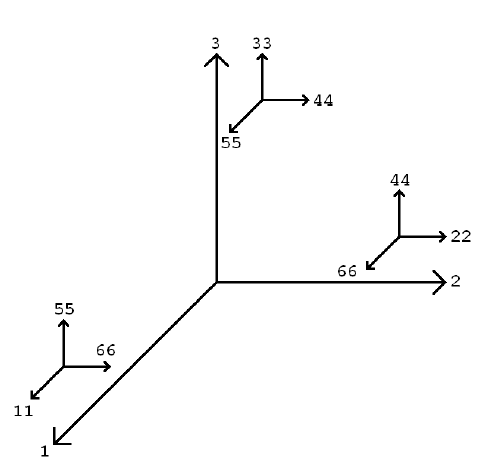
\includegraphics[width=0.5\textwidth]{png/speeds.png}}
\caption{Скорости распространения продольной и двух поперечных волн для каждой квазиодномерной волны.}
\label{pic:speeds-waves}
\end{figure}

\subsubsection{Трансверсальньно изотропное тело}
	
	Следующий тип анизотропии предполагает наличие во всех точках параллельных плоскостей упругой симметрии\cite{lehnitsky}.
	Иначе говоря, в каждой точке есть плоскость все направления в которой эквивалентны, а также есть выделенное направление, нормальное к плоскости.
	
	Примем за выделенное направление множество векторов коллинеарных оси $Z$, тогда плоскости изотропии будут параллельны плоскости $XY$.
	Матрица упругих постоянных имеет в этом случае всего пять независимых компонент:
\begin{align}
\label{vert_trans_tensor}
\left( \begin{array}{cccccccccccc}
c_{11} & c_{12} & c_{13} & 0 & 0 & 0 \\ 
c_{12} & c_{11} & c_{13} & 0 & 0 & 0 \\ 
c_{13} & c_{13} & c_{33} & 0 & 0 & 0 \\ 
0 & 0 & 0 & c_{44} & 0 & 0 \\ 
0 & 0 & 0 & 0 & c_{44} & 0 \\ 
0 & 0 & 0 & 0 & 0 & c_{66}
\end{array} \right){}
\end{align}
	где компоненты $c_{11}$, $c_{12}$, $c_{66}$ связаны соотношением:
\begin{equation}
	c_{66} = \frac{c_{11} - c_{12}}{2}.
\end{equation}

	Тензор упругих постоянных в этом случае похож на его аналог для орторомбической анизотропии, но тут он имеет меньшее количество независимых компонент.
	Это значит, что матрицы $\mathbf{A}_x$, $\mathbf{A}_y$, $\mathbf{A}_z$, а значит и собственные значения и собственные строки, имеют вид \eqref{orthorombic_mat1}-\eqref{orthorombic_mat3} с той лишь разницей, что некоторые компоненты зависимы и выражаются через другие.
	
	Данный вид анизотропии типичен для гексагональных решёток, а также для матрицы, аримированной однонаправленными волокнами -- основы ПКМ.
	
\subsection{Преобразование тензора упругих постоянных при повороте базиса}
	
	Многослойные ПКМ состоят из одинаковых слоёв, по-разному ориентированных вокруг оси укладки композита.
	Для расчёта конструкций необходимо найти вид тензора упругих постоянных в произвольно ориентированном базисе \cite{favorskaya}.
	
	Пусть $\theta_{x}$, $\theta_{y}$, $\theta_{z}$ -- углы поворота вокруг осей $x$, $y$, $z$ соответственно. 
	Чтобы перейти от старого базиса к новому нужно произвести последовательно эти повороты.
	Матрицы поворота будут иметь вид:
\begin{align}
\label{rotation_mat1}
\mathbf{G}_x =
\left( \begin{array}{cccccccccccc}
1 & 0 & 0 \\ 
0 & \cos \theta_{x} & -\sin \theta_{x} \\ 
0 & \sin \theta_{x} & \cos \theta_{x}
\end{array} \right),
\end{align} 
\begin{align}
\label{rotation_mat2}
\mathbf{G}_y =
\left( \begin{array}{cccccccccccc}
\cos \theta_{y} & 0 & \sin \theta_{y} \\
0 & 1 & 0 \\ 
-\sin \theta_{y} & 0 & \cos \theta_{y} 
\end{array} \right),
\end{align}
\begin{align}
\label{rotation_mat3}
\mathbf{G}_z =
\left( \begin{array}{cccccccccccc}
\cos \theta_{z} & -\sin \theta_{z} & 0 \\ 
\sin \theta_{z} & \cos \theta_{z} & 0 \\  
0 & 0 & 1  
\end{array} \right).
\end{align}
	
	Итоговая матрица преобразования базиса $\mathbf{G} = \mathbf{G}_{x}\mathbf{G}_{y}\mathbf{G}_{z}$ имеет вид:
\begin{align}
\label{rotation_mat}
\left( \begin{array}{cccccccccccc}
\cos \theta_{y} \cos \theta_{z} & \cos \theta_{z} \sin \theta_{x} \sin \theta_{y} - \sin \theta_{z} \cos \theta_{x} & \cos \theta_{x} \sin \theta_{y} \cos \theta_{z} + \sin \theta_{x} \sin \theta_{z} \\ 
\cos \theta_{y} \sin \theta_{z} & \sin \theta_{z} \sin \theta_{x} \sin \theta_{y} + \cos \theta_{z} \cos \theta_{x} & \cos \theta_{x} \sin \theta_{y} \sin \theta_{z} - \sin \theta_{x} \cos \theta_{z} \\ 
- \sin \theta_{y} & \sin \theta_{x} \cos \theta_{y} & \cos \theta_{x} \cos \theta_{y}
\end{array} \right)
\end{align}


	В итоге, тензор упругих постоянных $C_{ijkl}$, обсуждаемый в пункте 2.1, при поворотах системы координат будет преобразовываться по закону:
\begin{align}
	C_{mnpq} = \sum_{i,\;j,\;k,\;l = 1}^{3} g_{mi}\;g_{nj}\;g_{pk}\;g_{ql}\;C_{ijkl},
\end{align}
	где $g_{ij}$ -- тензор поворота, соответствующий матрице $\mathbf{G}$.

\clearpage
\newpage
\section*{Глава 3\\Численный метод}
\addcontentsline{toc}{section}{Глава 3. Численный метод}
\setcounter{section}{3}
\setcounter{subsection}{0}
\setcounter{equation}{0}

\subsection{Расщепление по направлениям}

	Чтобы решить систему уравнений:
\begin{equation}
	\label{matrix_anisotropy_equation1}
	\frac{\partial\vec{u}}{\partial{t}}+\mathbf{A}_x\frac{\partial\vec{u}}{\partial{x}}+
	\mathbf{A}_y\frac{\partial\vec{u}}{\partial{y}}+
	\mathbf{A}_z\frac{\partial\vec{u}}{\partial{z}}=0
\end{equation}
	методом конечных разностей потребывалось записать бы это уравнение на некотором сеточном шаблоне в каждом узле сетки, а затем решать полученную линейную систему.
	Решение этой системы, состоящей из огромного количества переменных представляется очень сложной задачей.
	С другой стороны вид системы \eqref{matrix_anisotropy_equation1} позволяет нам применить метод дробных шагов для её решения, сводя её, таким образом, к одномерной постановке:
\begin{equation}
	\label{norm_form}
	\frac{\partial\vec{u}}{\partial{t}}+\mathbf{A}_x\frac{\partial\vec{u}}{\partial{x}} = 0
\end{equation}

	Запишем для уравнения \eqref{norm_form} соотношение между искомым вектором на следующем временном слое $\vec{u}^{n+1}$ и на текущем $\vec{u}^{n}$ через оператор перехода между слоями $f$ в виде:
\begin{equation}
	\label{simple_splitting}
	\vec{u}^{n+1} = f_x(\mathbf{A}_x)\vec{u}^{n}.
\end{equation}	
	
	Тогда, в простейшем случае, окончательные выражение для $\vec{u}^{n+1}$ будет:
\begin{equation}
	\label{simple_3D_splitting}
	\vec{u}^{n+1} = F(\mathbf{A}_x, \mathbf{A}_y, \mathbf{A}_z)\vec{u}^{n},
\end{equation}
\begin{equation}
	\label{simple_3D_split_operator}
	F(\mathbf{A}_x, \mathbf{A}_y, \mathbf{A}_z) = \alpha_x f_x(\frac{\mathbf{A}_x}{\alpha_x}) + \alpha_y f_y(\frac{\mathbf{A}_y}{\alpha_y}) + \alpha_z f_z(\frac{\mathbf{A}_z}{\alpha_z}).
\end{equation}
	
	При условии, что за $f_x$, $f_y$, $f_z$ взяты разностные схемы, аппроксимирующие соответствующие уравнения вида \eqref{norm_form}, как минимум первого порядка точности по пространству, а также при выполнении условия:
\begin{equation}
	\label{simple_3D_split_cond}
	\alpha_x + \alpha_y + \alpha_z = 1, \quad \alpha_x, \alpha_y, \alpha_z > 0,
\end{equation}
	схема \eqref{simple_3D_splitting} с оператором \eqref{simple_3D_split_operator} обеспечивает первый порядок точности.
	Такой подход, комбинирующий сочетания решений одномерных систем, носит название \textit{расщепление по направлениям} \cite{chelnokov}.
	
	Ограничение на шаг по времени $\tau$, обеспечивающее устойчивость дальнейшего численного решения, будет иметь вид:
\begin{equation}
\tau \le \max{\tau_j} = \frac{\min(h)}{\max(|\lambda_j^*|)} = \frac{\min(h)\alpha_j}{\max(|\lambda_j|)},
\end{equation}
	где $\lambda_j$ -- собственные значения матриц $\mathbf{A}_x$, $\mathbf{A}_y$, $\mathbf{A}_z$.
	
	Если за одномерные операторы перехода $f$ взять схемы второго порядка и скомбинировать их в полный оператор:
\begin{equation}
	\label{3D_split_operator}
	F(\mathbf{A}_x, \mathbf{A}_y, \mathbf{A}_z) = \frac{1}{6}\sum_{i \neq j \neq k \neq i} f_i(\mathbf{A}_i)f_j(\mathbf{A}_j)f_k(\mathbf{A}_k),
\end{equation}
	то мы получим схему второго порядка. 
	
	Допустимый шаг по времени определяется минимальным допустимым шагом по времени для схем $f_j$:
\begin{align}
\tau = \min\limits_{j}(\tau_j) = \min\limits_{j}(\frac{\min(h)}{\max(|\lambda_j|)}) = \frac{\min(h)}{\max\limits_{j}\max(|\lambda_j|)}.
\end{align}
	
	Однако вычисления по схеме \eqref{3D_split_operator} требуют больших затрат компьютерного времени и памяти.
	Как оказалось, вычисление любого одного слагаемого из \eqref{3D_split_operator} даёт хорошее приближение к схеме второго порядка, например:	
\begin{equation}
	\label{short_3D_split_operator}
	F(\mathbf{A}_x, \mathbf{A}_y, \mathbf{A}_z) = f_x(\mathbf{A}_x)f_y(\mathbf{A}_y)f_z(\mathbf{A}_z).
\end{equation}
	
\subsection{Гиперболическая система уравнений. Инварианты Римана}
	
	Систему квазилинейных уравнений в частных производных, записанную в \textit{нормальной форме} \eqref{norm_form} будем считать \textit{гиперболической}.
	Это значит, что матрица $\mathbf{A}$ подчиняется условиям\cite{rozhdestvenskiy}:
\begin{itemize}
	\item все собственные значения матрицы $\lambda_{i} = \lambda_{i}(t, x, \vec{u})$, $i = \overline{1, 9}$ вещественны;
	\item система собственных векторов матрицы $\{l_{i}(t, x, \vec{u})\}$, $i = \overline{1, 9}$ образует базис в пространстве $E_{n}$.
\end{itemize}

	В таком случае матрица $\mathbf{A}$ \textit{диагонализуема}, т.е. существует базис -- басиз собственных векторов -- в котором она имеет диагональный вид.
	Тут мы будем говорить о собственных строках $\vec{l}^{T}$, таких, что:
\begin{equation}
	\label{eigenstr_equation}
	\vec{l}^{T}\mathbf{A} = \lambda\vec{l}^{T}.
\end{equation}
	
	Итак, матрица $\mathbf{A}$ представима в виде:
\begin{equation}
	\label{diagonal_view}
	\mathbf{A} = \mathbf{\Omega}^{-1}\mathbf{\Lambda}\mathbf{\Omega},
\end{equation}	
	где $\mathbf{\Omega}$ -- матрица собственных строк, $\mathbf{\Lambda}$ -- диагональная матрица собственных значений.
	Тогда умножая справа \eqref{norm_form} на $\mathbf{\Omega}$ получим:
\begin{equation}
	\label{norm_form1}
	\mathbf{\Omega}\frac{\partial\vec{u}}{\partial{t}}+\mathbf{\Lambda}\mathbf{\Omega}\frac{\partial\vec{u}}{\partial{x}} = 0.
\end{equation}
	Далее, если компоненты матрицы $\mathbf{\Omega}$ не зависят от переменных $(x, t)$, то её можно внести под знак дифференцила:
\begin{equation}
	\label{norm_form2}
	\frac{\partial(\mathbf{\Omega}\vec{u})}{\partial{t}}+\mathbf{\Lambda}\frac{\partial(\mathbf{\Omega}\vec{u})}{\partial{x}} = 0.
\end{equation}
	В общем случае, когда $\mathbf{\Omega} = \mathbf{\Omega}(x, t, \vec{u})$, $\mathbf{\Lambda} = \mathbf{\Lambda}(x, t, \vec{u})$ можно попробывать поискать интегрирующий множитель, однако для системы девяти уравнений это проблематично.
	
	Обозначая, $\vec{r} = \mathbf{\Omega}\vec{u}$ получим уравнение:
\begin{equation}
	\label{Riman_invariantes}
	\frac{\partial\vec{r}}{\partial{t}}+\mathbf{\Lambda}\frac{\partial\vec{r}}{\partial{x}} = 0.
\end{equation}
	Или же в такой форме \cite{kukudzhanov_main}:
\begin{equation}
	\label{Riman_invariantes1}
	\left(\frac{dr_k}{dt}\right)_k = 0, \quad k = \overline{1, 9},
\end{equation}
	где $r_k$, компоненты вектора $\vec{r}$ называются \textit{инвариантами Римана}, а система \eqref{Riman_invariantes} \textit{системой в инвариантах}.
	В записи \eqref{Riman_invariantes} введено обозначение:
\begin{equation}
	\label{notation}
	\left(\frac{d}{dt}\right)_k = \frac{\partial}{\partial{t}} + \lambda_k \frac{\partial}{\partial{x}}
\end{equation}
	Это оператор дифференцирования вдоль направления, заданного уравнением:
\begin{equation}
	\label{characteristic_direction}
	\frac{dx}{dt} = \lambda_k, \quad k = \overline{1, 9}.
\end{equation}
	Уравнения \eqref{characteristic_direction} -- уравнения на \textit{характеристики} системы \eqref{norm_form} -- интегральные кривые вдоль которых инварианты $r_k$ постоянны. 
	
	Эти рассуждения лежат в основе \textit{метода характеристик} -- метода решения систем гиперболических уравнений, в котором решение уравнений в частных производных сводится к решению обыкновенных дифференциальных уравнений (ОДУ).
	В свою очередь, для численного решения ОДУ могут быть применены стандартные конечно-разностные схемы. Такой подход составляет суть \textit{сеточно-характеристического метода}. 
	
\subsection{Cеточно-характериситческий метод}

	Гиперболические уравнения описывают распространение различного типа волн в средах.
	Простейшим решением одномерного волнового уравнения являются две волны: $f(x \pm vt)$, распространяющиеся в противоположных направлениях.
	Функция $f$ -- вид начального возмущения, как можно видеть, параметризованная указаным образом, она даёт решение уравнения.
	Важным здесь является то, что некоторые линейные комбинации искомых величин сохраняются на определённых пространственно-временных кривых (характеристиках).

\begin{figure}[H]
	\center{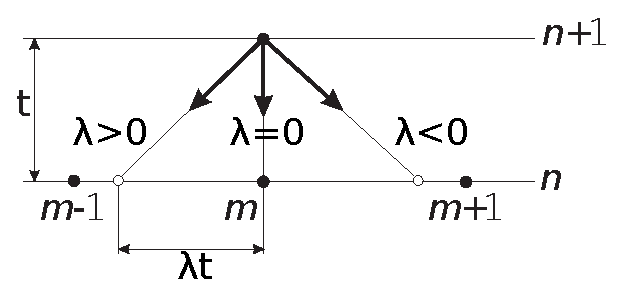
\includegraphics[width=0.5\textwidth]{png/gcm-idea.eps}}
	\caption{Принципиальная схема сеточно-характеристического метода.}
\end{figure}

	После расщепления наша система предстаёт в виде трёх гиперболических систем, описывающих распространение продольной и двух поперечных волн вдоль каждой оси (всего вдоль каждой оси распространяется шесть волн -- с положительными и отрицательными скоростями).
	Затем, переходя к инвариантам, мы получаем девять уравнений переноса вдоль каждой оси.
	Решение этих уравнений сеточно-характеристическим методом осуществляемся следующим образом:
\begin{enumerate}
	\item Из узлов сетки на очередном временном слое проводятся характеристики на предыдущий временной слой (см. Рис. 2). Для линейной системы уравнений характеристиками будут семейства параллельных прямых.
	\item Находятся точки пересечения характеристик с предыдущим временным слоем.
	\item В этих точках, применяя различные схемы, производится интерполяция искомых функций (на Рис. 2 изображён трёхточечный шаблон).
	\item По найденным значениям производится пересчёт инвариантов, которые переносятся по характеристикам в исходный узел.
\end{enumerate}
	
	Как уже сказано характеристики -- прямые линиии постоянного наклона. Это значит можно точно решить уравнение на характеристики \eqref{characteristic_direction}, поэтому определяющим фактором здесь является интреполяция инвариантов.
	Схема интерполяции второго порядка с разностями против потока (upwind scheme) является здесь предпочтительной.
	При числе Куранта в близкой окрестности единицы эта схема может оказаться особенной точной.
	
	В итоге инварианты на $(n+1)$-ом временном слое можно записать в виде:
\begin{equation}
	r_{i}^{n+1} = r_{i}^{n}(- \lambda_{i}\tau),
\end{equation}
	где $r_{i}$ -- $i$-ый инвариант Римана, $\lambda_{i}$ -- соответствующее ему собственное значение.
	Такая запись означает, что значение инварианта $r_{i}$ берётся на $n$-ом слое в точке смёщённой на $-\lambda_{i}\tau$ от координаты искомой.
	
	Затем искомый $\vec{u}$ вектор находится по формуле:
\begin{equation}
	\vec{u} = \mathbf{\Omega^{-1}}\vec{r}.
\end{equation}	

\subsection{Разностные схемы для структурированных сеток}
	
	Существует множество готовых расностных схем для решения уравнения \eqref{norm_form}.
	По сути эти схемы аналогичны сеточно-характерестическому методу, использующему различные схемы интерполяции инвариантов на предыдущем слое.
	
\paragraph{Схема Куранта-Изаксона-Рис.} Данная схема строится на трёхточечном сеточном шаблоне $(m-1, m, m+1)$ и позволяет явно выразить значение $\vec{u}_m^{n+1}$ на новом временном слое:
\begin{equation}
	\label{CIR scheme}
	\vec{u}^{n+1}_m = \vec{u}^n_m - \frac{\tau}{h} \mathbf{\Omega}^{-1} \mathbf{\Lambda}^+ \mathbf{\Omega} (\vec{u}^n_{m+1} - \vec{u}^n_m) 
	- \frac{\tau}{h} \mathbf{\Omega}^{-1} \mathbf{\Lambda}^- \mathbf{\Omega} (\vec{u}^n_m - \vec{u}^n_{m-1}) .
\end{equation}
	Здесь диагональные матрицы $\mathbf{\Lambda}^+$, $\mathbf{\Lambda}^-$ содержат соответственно положительные и отрицательные собственные значения (скорости распространения волн).
	
	Эта схема является схемой первого порядка точности по времени и пространству -- $O(h, \tau)$.
	
\paragraph{Схема Лакса-Вендрофа.} Стандартная схема Лакса-Вендрофа обладает вторым порядком точности и по времени и по пространству -- $O(h^2 + \tau^2)$.
\begin{equation}
	\label{LW scheme}
	\vec{u}^{n+1}_m = \vec{u}^n_m - \frac{\tau}{2h} \mathbf{A} (\vec{u}^n_{m+1} - \vec{u}^n_{m-1})
	 + \frac{\tau^2}{2h^2} \mathbf{A}^2 (\vec{u}^n_{m+1} - 2\vec{u}^n_m + \vec{u}^n_{m-1}) .
\end{equation}
	Эта схема в отличие от предыдущей не является монотонной. 
	Схемы, у которых отсутствует свойство монотонности плохо аппроксимируют решения с большими градиентами -- они выдают осцилляции разностного происхождения вблизи области с больши градиентом.
	
\paragraph{Гибридная схема.} Именно для сочетания точности схем второго порядка и устранения осцилляций для решений с большими градиентами Р.П. Федоренко впервые предложил \textit{гибридные схемы} \cite{fedorenko}.
	В нашем случае, комбинируя схему \eqref{CIR scheme} со схемой \eqref{LW scheme}, итоговое решение будет иметь вид линейной комбинации решений двух схем:
\begin{align}
	\label{hybrid scheme}
	\vec{u}^{n+1}_m &= \vec{u}^n_m - \frac{\tau}{2h} \mathbf{A} (\vec{u}^n_{m+1} - \vec{u}^n_{m-1}) + \nonumber\\
		&+ \frac{1}{2} ((1-a) \frac{\tau}{h} \mathbf{\Omega}^{-1} |\mathbf{\Lambda}| \mathbf{\Omega} + a \frac{\tau^2}{h^2} \mathbf{A}^2 ) (\vec{u}^n_{m+1} - 2\vec{u}^n_m + \vec{u}^n_{m-1}).
\end{align}
	Параметр $a$ может принимать значения: $0 \leq a \leq 1$, и подбирается на каждом шагу в зависимости от степени гладкости решения. 
	В случае $a = 0$ схема \eqref{hybrid scheme} переходит в схему Куранта-Изаксона-Рис \eqref{CIR scheme}.
	В случае $a = 1$ схема \eqref{hybrid scheme} переходит в схему Лакса-Вендрофа \eqref{LW scheme}.
	
	Решение уравнения \eqref{norm_form} по схеме \eqref{hybrid scheme} заключается в переключении между схемами \eqref{CIR scheme} и \eqref{LW scheme} в зависимости от гладкости $n$-ого временного слоя.
	Критерий переключения имеет вид:
\begin{equation}
	\label{Fedorenko criterium}
	\left|\frac{\vec{u}^n_{m+1} - 2\vec{u}^n_m + \vec{u}^n_{m-1}}{\vec{u}^n_{m+1} - \vec{u}^n_{m-1}}\right| \le K,
\end{equation}
	где параметр переключения -- $K$ подбирается, опять же, в зависимости от гладкости решения и в данной работе: $K = 0.5$.
	В случае выполнения условия \eqref{Fedorenko criterium} решение считается достаточно гладким, параметр принимает значение: $a = 1$ и расчёт ведётся по схеме Лакса-Вендрофа.
	Если же критерий не выполняется, то $a = 0$ и расчёт производится по схеме Куранта-Изаксона-Рис.
	
	На Рис. 3 изображены несколько численных решений распространения прямоугольного импульса. Как можно отметить гибридная схема лучше остальных приближает точное решение.
\begin{figure}[H]
\centerline{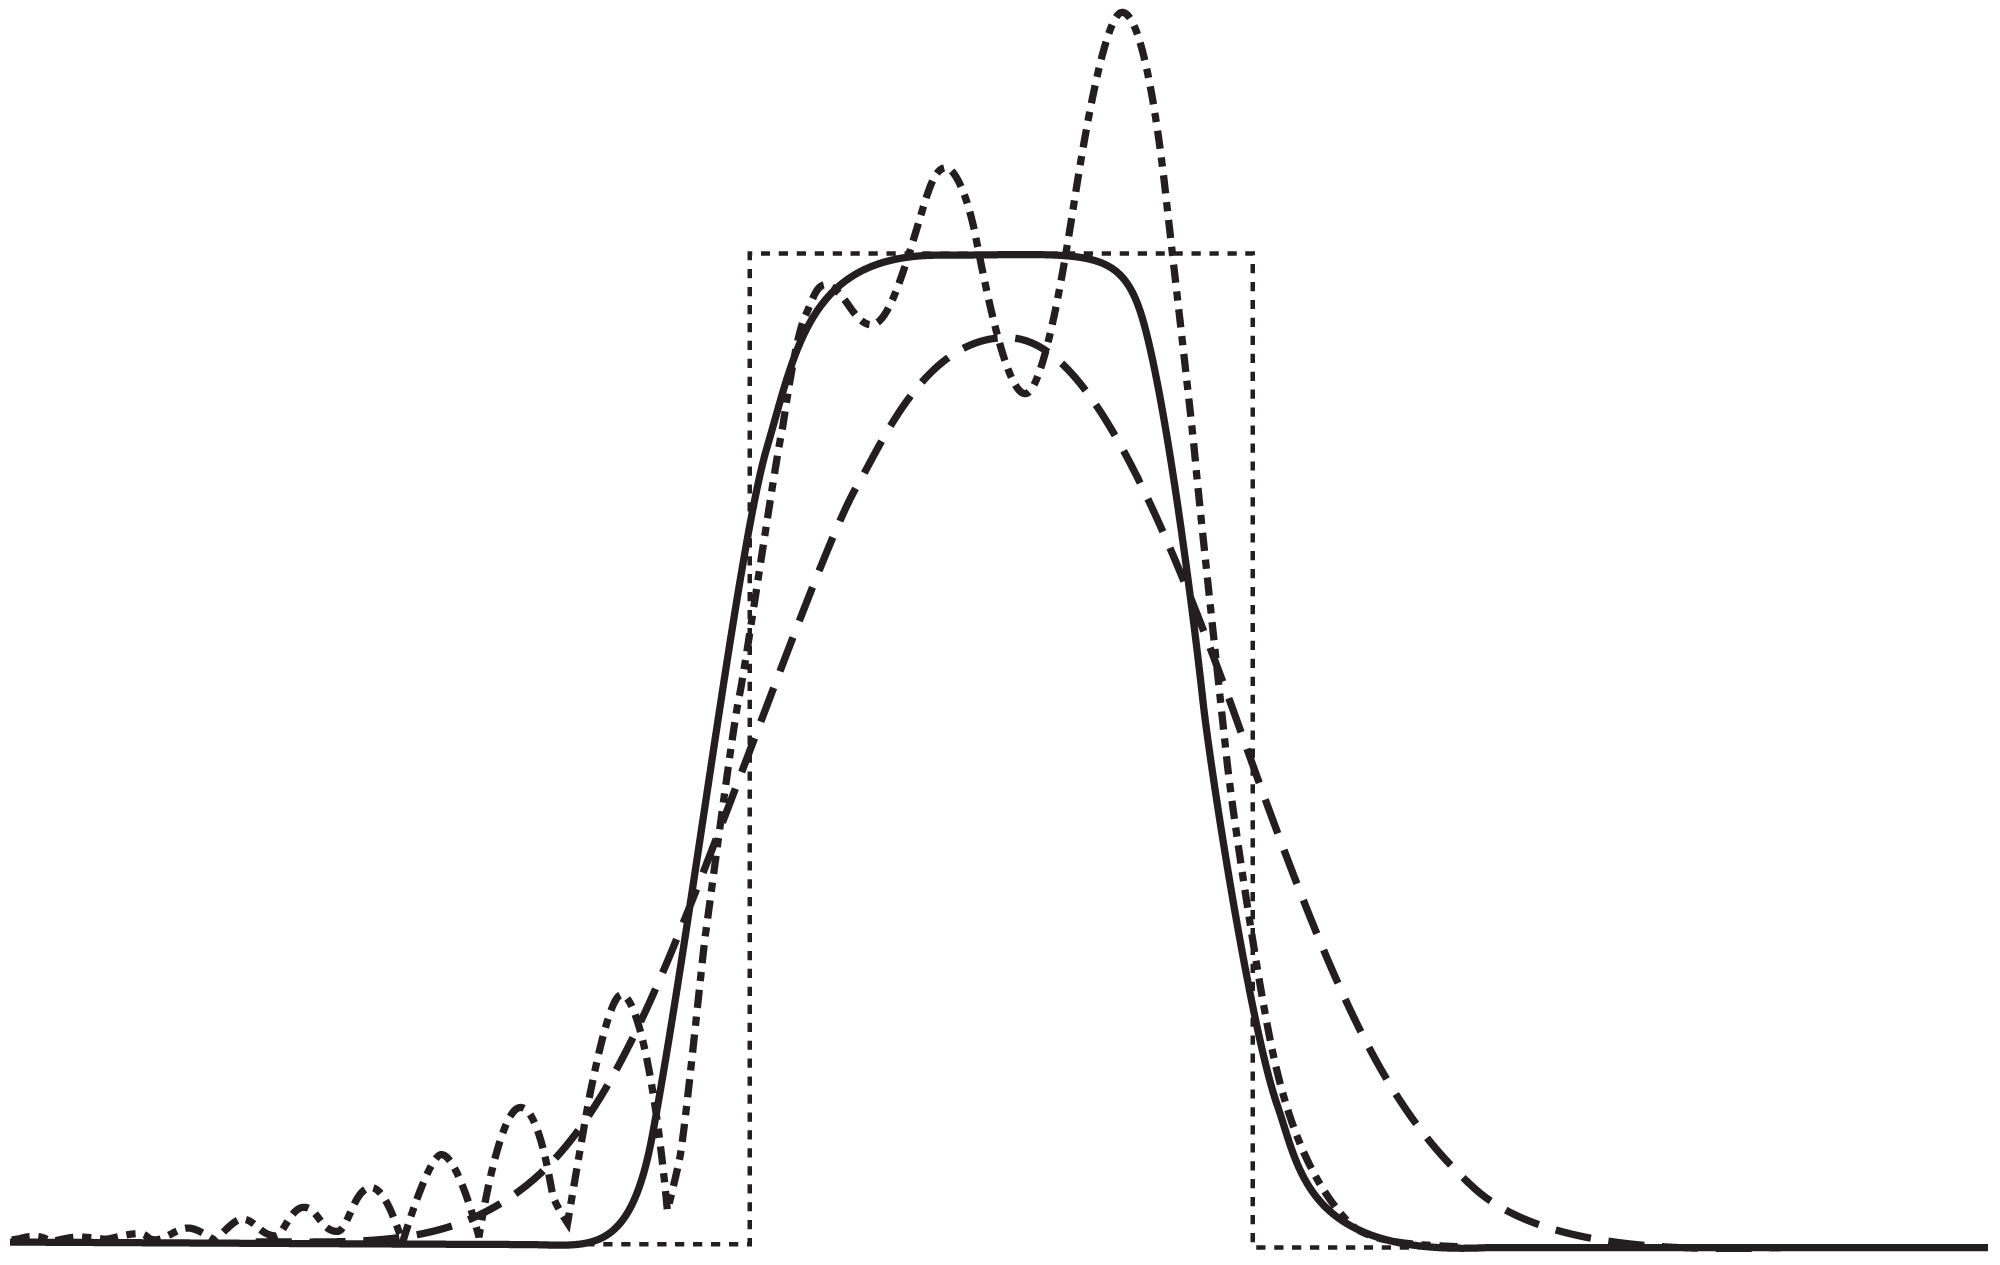
\includegraphics[width=0.75\textwidth]{png/hybrid-scheme-testing.png}}
\caption{Распространение прямоугольного импульса. Штриховая линия -- решение по схеме Куранта-Изаксона-Рис. Штрих-пунктирная -- решение по схеме Лакса-Вендрофа. Сплошная линия -- решение с использованием гибридной схемы. Точками показано точное решение.}
\label{pic:hybrid-scheme-testing}
\end{figure}

\clearpage
\newpage
\newpage
\section{Полученные результаты}
\subsection{Расчёты в }
\subsubsection{Линейная упругость}

\clearpage
\newpage
\section{Заключение}
Результаты, полученные в результате выполнения дипломного проекта:
\begin{itemize}
\item Рассмотрены различные подходы к описанию движения сплошной среды в сочетании с применяемыми к ним численными методами
\item Предложен метод моделирования сплошной среды в 1D с учётом движения и деформации тела, в том числе схема второго порядка точности по координате с учётом изменения характеристик среды в пространстве, точная со вторым порядком по времени схема расщепления рассчётного шага на движение рассчётной сетки и перенос возмущения
\item На основе данного метода реализован программный комплекс, моделирующий деформируемое твёрдое тело в случае одного пространственного измерения с поддержкой упругой и упругопластической реологии
\item Проведено сравнение результатов работы данного программного комплекса с результатами полуаналитического рассчёта на основе принципиально другого подхода к описанию сплошной среды и итерационного  метода. Получена сходимость результатов со вторым порядком точности по времени и координате
\item Предложен способ моделирования идеально-пластической реологии в 3D на основе правила корректировки Уилкинса
\item Данный способ реализован на основе существующего программного комплекса, поддерживающего линейную упругость в 3D
\item Проведено сравнение результатов. Получено удовольствие
\end{itemize}

\clearpage
\newpage
\begin{thebibliography}{99}
\addcontentsline{toc}{section}{Литература}
\bibitem{kukudganov}Кукуджанов В.Н. Вычислительная механика сплошное сред. - М.: Издательство 
Физико-математической литературы, 2008, с. 32, с. 242, с. 271.
\bibitem{resler}И.Реслер, Х.Хардерс, М.Бекер Механическое поведение конструкционных материалов. Перевод с немецкого. - Долгопрудный, Издательский дом <<Интеллект>>, 2011, с. 91-115
\bibitem{novatsky}Новацкий В. К. Теория упругости. — М. : Мир, 1975, c. 105-107.
\bibitem{sedov}Седов Л. И. Механика сплошной среды. Том 1. — М. : Наука, 1970, с. 143.
\bibitem{rebotnov}Работнов Ю.Н. Механика деформируемого твёрдого тела. — М.: Наука, 1988. — 712 с.
\bibitem{belocerkovsky}Белоцерковский О.М. Численное моделирование в механике
сплошных сред. — М.: Физико-математическая литература. 1994, 442 с.
\bibitem{magomedov}Магомедов К.М., Холодов А.С. Сеточно-характеристические
численные методы. — М.: Наука, 1988, 288 с.
\bibitem{holodov}Холодов А.С., Холодов Я.А. О критериях монотонности разностных
схем для уравнений гиперболического типа. 
\bibitem{chelnokov}Челноков Ф.Б. Численное моделирование деформационных
процессов в средах со сложной структурой.
\bibitem{fedorenko}Федоренко Р.П. Введение в вычислительную физику. М.:
Изд-во Моск. физ. -техн. ин-та, 1994, 528 с.
\bibitem{chushkin}Чушкин П.И. Метод характеристик для пространственных сверхзвуковых течений. –  Труды ВЦ АН СССР, 1968, c. 121.
\bibitem{petrov_chelnokov}Петров И.Б., Челноков Ф.Б. Численное исследование волновых процессов и процессов разрушения в многослойных преградах // Журнал вычислительной математики и математической физики – 2003, том 43, N 10, с. 1562-1579.
\bibitem{matyushev_petrov}Matyushev N.G., Petrov I.B. Mathematical Simulation of Deformation and Wave Processes in Multilayered Structures // Computational Mathematics and Mathematical Physics – 2009, Vol. 49, N 9, P. 1615-1621.
\bibitem{petrov_tormasov_holodov}Петров  И.Б., Тормасов А.Г., Холодов А.С. О численном изучении нестационарных процессов в деформируемых средах многослойной структуры // Механика твердого тела – 1989, N 4, с. 89-95.
\bibitem{golubev_kvasov_petrov}Голубев В.И., Квасов И.Е., Петров И.Б. Воздействие природных катастроф на наземные сооружения // Математическое моделирование – 2011, том 23, N 8, с. 46-54.
\bibitem{agapov_belocerkovsky_petrov}Агапов П.И., Белоцерковский О.М., Петров И.Б. Численное моделирование последствий механического воздействия на мозг человека при черепно-мозговой травме // Журнал вычислительной математики и математической физики – 2006, том 46, N 9, с. 1711-1720.
\bibitem{petrov}Петров И.Б. Волновые и откольные явления в слоистых оболочках конечной толщины // Механика твердого тела – 1986, N 4, с. 118-124.
\end{thebibliography}

\end{document}
